\documentclass[preprint,12pt,authoryear]{elsarticle}

\usepackage[utf8]{inputenc}
\usepackage[T1]{fontenc}
\usepackage{amsmath,amssymb,amsthm}
\usepackage{array,booktabs,longtable,multirow,tabularx,threeparttable}
\usepackage{float}
\usepackage{graphicx}
\usepackage{hyperref}
\usepackage{microtype}
\usepackage{xcolor}
\usepackage{tikz}
\usetikzlibrary{arrows.meta,calc,fit,positioning}

\graphicspath{{paper/images/}}
\newcolumntype{Y}{>{\raggedright\arraybackslash}X}
\DeclareMathOperator*{\argmax}{arg\,max}
\DeclareMathOperator*{\argmin}{arg\,min}

\definecolor{tabblue}{HTML}{1F77B4}
\definecolor{taborange}{HTML}{FF7F0E}
\definecolor{tabgreen}{HTML}{2CA02C}
\definecolor{tabred}{HTML}{D62728}
\definecolor{tabpurple}{HTML}{9467BD}
\definecolor{tabbrown}{HTML}{8C564B}
\definecolor{tabpink}{HTML}{E377C2}
\definecolor{tabgray}{HTML}{7F7F7F}
\definecolor{tabolive}{HTML}{BCBD22}
\definecolor{tabcyan}{HTML}{17BECF}
\definecolor{journalbg}{HTML}{F7F8FA}
\definecolor{journalline}{HTML}{5A5A5A}
\definecolor{journalgrid}{HTML}{D9D9D9}

\setlength{\textfloatsep}{10pt plus 2pt minus 2pt}
\setlength{\floatsep}{8pt plus 2pt minus 2pt}
\setlength{\intextsep}{10pt plus 2pt minus 2pt}
\setlength{\abovecaptionskip}{5pt}
\setlength{\belowcaptionskip}{0pt}

\tikzset{
every picture/.style={line cap=round,line join=round},
>={Latex[length=2.4mm,width=1.6mm]},
journal box/.style={
  draw=journalline,
  rounded corners=2.5pt,
  line width=0.7pt,
  minimum height=1.0cm,
  align=center,
  inner sep=4pt,
  fill=journalbg,
  font=\footnotesize
},
journal group/.style={
  draw=tabgray,
  dashed,
  rounded corners=4pt,
  line width=0.7pt,
  inner sep=6pt
},
fig flow/.style={
  draw=journalline,
  -{Latex[length=2.2mm,width=1.5mm]},
  line width=0.95pt
},
fig dashed/.style={
  draw=tabgray,
  -{Latex[length=2.2mm,width=1.5mm]},
  line width=0.9pt,
  dash pattern=on 3pt off 2pt
},
fig label/.style={font=\footnotesize, text=black!80, align=center},
grid line/.style={draw=journalgrid, line width=0.5pt},
home node/.style={draw=tabblue!75!black, fill=tabblue!10, rounded corners=2pt, line width=0.7pt},
mp node/.style={draw=taborange!85!black, fill=taborange!10, rounded corners=2pt, line width=0.7pt},
vehicle node/.style={draw=tabgreen!70!black, fill=tabgreen!10, rounded corners=2pt, line width=0.7pt},
cbd node/.style={draw=tabpurple!75!black, fill=tabpurple!9, rounded corners=2pt, line width=0.7pt},
soft blue box/.style={journal box, fill=tabblue!8},
soft orange box/.style={journal box, fill=taborange!8},
soft green box/.style={journal box, fill=tabgreen!8},
soft red box/.style={journal box, fill=tabred!8},
soft purple box/.style={journal box, fill=tabpurple!8},
soft cyan box/.style={journal box, fill=tabcyan!8},
soft gray box/.style={journal box, fill=black!2}
}

\journal{Transportation Research Part C: Emerging Technologies}

\begin{document}

\begin{frontmatter}

\title{Smart Predict-Then-Optimize for Dynamic Meeting-Point Recommendation and Pricing in Many-to-One Demand-Responsive Transit}

\author[aff1]{Jin An}
\author[aff1]{Tian-Liang Liu}
\author[aff1]{Guanghui Fu}

\address[aff1]{MoE Key Laboratory of Complex System Analysis and Management Decision, School of Economics and Management, Beihang University, Beijing 100191, China}

\begin{highlights}
\item A sequential DRT model is formulated for home pickup, meeting points, and endogenous quitting.
\item DRPO extends DSPO with an SPO+-based decision-focused learning objective.
\item Synthetic and Beijing experiments show consistent gains over DSPO and competitive cost outcomes.
\end{highlights}

\begin{abstract}
Demand-responsive transit (DRT) can complement fixed-route public transport, but a purely door-to-door service pattern often entails high operating costs, substantial detours, and unstable service quality. This paper studies a many-to-one DRT setting in which passengers arrive sequentially during the booking horizon and may choose between home pickup and nearby meeting points. To support these choices, it proposes the Dynamic meeting-point Recommendation and Pricing Optimization (DRPO) framework, which adapts the original DSPO pipeline to DRT and augments it with a Smart Predict-Then-Optimize (SPO) decision-focused training objective. For each arriving passenger, the operator offers a menu consisting of home pickup and recommended meeting points, with each option characterized by a fare, a walking distance, and a predicted in-vehicle travel time. The online problem is formulated as a Markov decision process in which the offered set is generated heuristically and the pricing vector is optimized conditional on that set. To make the problem tractable, the downstream routing impact of each boarding option is approximated through predicted marginal insertion costs, and the prediction module is trained with a blended Huber/SPO+ objective aligned with downstream pricing decisions. Empirically, DRPO is benchmarked against six policies on a synthetic instance family and against Static-pricing, DSPO, and DRPO on a semi-realistic Beijing case, with seed-level means and dispersion measures reported throughout. In the synthetic benchmark, DRPO reduces mean total cost by 12.14\% relative to Static-pricing and improves mean net profit by 6.94\% over DSPO. In the Beijing 25-vehicle case, DRPO improves net profit on all five matched seeds, reduces mean total cost by 1.35\% relative to DSPO and by 1.62\% relative to Static-pricing, and lowers the quit rate from 4.04\% to 3.24\%. Additional fleet-size and behavioral-sensitivity analyses indicate that the relative benefit of DRPO depends on passenger price sensitivity and the attractiveness of the outside option. Overall, the results show that adding the SPO framework to DSPO improves the learning-based pricing policy in the tested DRT settings without relying on aggressive passenger steering.
\end{abstract}

\begin{keyword}
demand-responsive transit \sep meeting-point recommendation \sep dynamic pricing \sep Smart Predict-Then-Optimize \sep many-to-one service
\end{keyword}

\end{frontmatter}

\section{Introduction}
\label{sec:intro}

Demand-responsive transit (DRT) occupies an intermediate position between fixed-route public transport and fully individualized travel. By adapting service provision to realized demand, DRT can improve accessibility in settings where travel demand is spatially dispersed, temporally uneven, and too thin to justify frequent fixed-route service. Many-to-one applications are especially common in practice, including commuter flows from suburban neighborhoods to central business districts and school-oriented services that consolidate riders from multiple origins to a common destination.

Two service patterns are widely used in current DRT systems. In a home-pickup service, vehicles provide door-to-door collection and passengers wait at their origins. In a meeting-point service, passengers walk to designated pickup locations and vehicles stop only when a booking is present. The first pattern improves convenience, but often at the cost of longer detours, higher vehicle mileage, and lower schedule reliability. The second pattern can reduce detours and simplify operations, yet an exclusive reliance on meeting points may weaken service attractiveness and reduce passenger acceptance. Prior studies show that meeting-point designs can improve reliability and operating efficiency when walking distances remain reasonable \citep{zheng2019,zhang2023routing}, but the literature provides less guidance on how operators should manage services when passengers may choose between home pickup and meeting points in real time.

This gap is consequential because boarding choices shape both operator-side efficiency and passenger-side service quality. A passenger's willingness to accept a meeting point depends not only on walking distance, but also on price and expected in-vehicle travel time \citep{bai2019}. In operational settings, however, these attributes must be communicated when the request is made, even though the final routing plan will only be known after all requests have been collected. The operator therefore faces a sequential decision problem in which current prices and displayed information affect future routing outcomes under uncertain demand.

This paper addresses that problem by proposing the Dynamic meeting-point Recommendation and Pricing Optimization (DRPO) framework for many-to-one DRT. DRPO is not introduced as an entirely new pricing architecture; rather, it adapts the original DSPO pipeline to a DRT setting with home pickup, meeting points, and endogenous quitting, and it adds an SPO-based decision-focused learning objective. In the codebase, this variant is implemented as \texttt{DSPO\_plus\_SPO}. For each arriving passenger, DRPO first constructs a feasible option set consisting of home pickup and nearby meeting points, and then determines option-specific price adjustments to balance demand steering and operational efficiency. The framework combines three elements: heuristic meeting-point recommendation, a passenger-choice model that captures responses to price, walking distance, and in-vehicle travel time, and decision-focused learning that trains the prediction module according to downstream pricing performance rather than prediction accuracy alone.

The paper makes three contributions: (i) it formulates a many-to-one DRT pricing problem in which the operator jointly manages home pickup, meeting-point recommendation, and the outside option under sequential passenger arrivals; (ii) it documents an implementation-oriented DRPO pipeline, including the meeting-point generation rule, calibrated service-time and utility parameters, and the SPO-augmented learning schedule used to turn DSPO into \texttt{DSPO\_plus\_SPO}; and (iii) it provides an expanded empirical assessment with six synthetic benchmark policies, a five-seed Beijing case study, matched-seed comparisons against DSPO, fleet-size checks, and behavioral-sensitivity analyses.

The remainder of the paper is organized as follows. Section~\ref{sec:related} reviews related literature. Section~\ref{sec:model} formulates the many-to-one DRT pricing problem. Section~\ref{sec:method} presents the DRPO methodology. Section~\ref{sec:results} reports numerical results for the synthetic benchmark and the semi-realistic Beijing case study. Section~\ref{sec:conclusion} concludes, Section~\ref{sec:data} gives the data-and-code-availability statement, and Appendix~\ref{app:addl} reports additional implementation details and supplementary experiments.

\section{Related work}
\label{sec:related}

The present study lies at the intersection of four research streams: DRT system design and operations, meeting-point-based and pricing-based demand steering, passenger-choice modeling, and decision-focused learning for downstream optimization.

\subsection{Demand-responsive transit systems}

Recent DRT research has examined system design, operational optimization, and service equity from multiple perspectives. On the system-design side, \citet{baier2024} provide a structured framework for evaluating DRT performance, while \citet{sorensen2021} and \citet{currie2020} show that fully flexible door-to-door services often struggle with high operating costs, especially in low-density or operationally complex environments. Recent empirical and policy-oriented studies likewise emphasize that deployment outcomes depend on local operating practice and commuting context \citep{ghimire2024,gerzinic2025}. These findings underscore a central tension in DRT: flexibility improves convenience, but can also undermine cost efficiency and reliability.

Operational optimization studies have sought to mitigate that tension through data-driven and algorithmic methods. \citet{lyu2019} and \citet{xia2022} develop route-planning approaches for customized bus systems, and \citet{wu2024} propose a multi-agent deep reinforcement learning framework for real-time route control. Related work also considers prediction and stochastic planning in flexible transport systems. For example, \citet{kostic2021} model idle-time prediction in shared mobility, \citet{lee2021} optimize zonal flexible bus services under stochastic demand, and \citet{liu2023} analyze customized public transport ridership using machine-learning and spatial methods. Collectively, these studies show that predictive and adaptive control methods can improve DRT performance, but they mostly focus on routing or supply-side planning rather than jointly modeling passenger boarding choices and sequential pricing.

\subsection{Meeting points, walking coordination, and pricing}

Meeting-point-based operations have received growing attention because they offer a way to improve routing efficiency without abandoning service flexibility altogether. \citet{zheng2019} show that introducing meeting points into flex-route transit can generate sizable operational benefits, and \citet{fielbaum2021} demonstrate that optimized walking locations can improve on-demand ridesharing performance. More recent work likewise shows that flexible stop assignment and walking-based coordination can improve efficiency in on-demand systems \citep{wu2025,zhang2025,li2025,pellegrini2025,yan2025}. Even so, most studies treat meeting-point assignment as a planning or control problem and pay limited attention to how real-time prices can be used to influence passenger acceptance of meeting points relative to home pickup.

Dynamic pricing has long been studied as a mechanism for balancing demand and operational costs under uncertainty. In logistics and delivery settings, \citet{galiullina2024} and \citet{akkerman2025} show that dynamic selection and pricing can steer demand toward more efficient service options. \citet{yang2016} demonstrate that pricing and routing decisions can be profitably coordinated in e-fulfillment, while \citet{dong2009} characterize optimal pricing under substitution effects. Beyond transportation, dynamic pricing has also been studied in retail, energy, and service operations \citep{kayikci2022,chen2017,zhao2021}. In DRT and adjacent mobility services, pricing has also been identified as a promising lever. \citet{wang2021} show that passenger incentives can reduce detours and improve operator profit, and \citet{li2021} study strategic pricing in customized bus and ride-sharing settings. Yet most of this work remains static or offline in nature, and it rarely models the sequential arrival of passengers together with the need to quote service attributes, such as in-vehicle travel time, before the downstream routing problem is fully realized.

\subsection{Passenger behavior and decision-focused learning}

Equity and user experience remain important concerns in the DRT literature. \citet{liezenga2024}, \citet{miller2016}, and \citet{shang2022} emphasize that DRT affects accessibility, affordability, and service inclusion, especially for vulnerable travelers. Other studies document heterogeneous willingness across user groups to adopt DRT services \citep{knierim2021}. These findings highlight the importance of explicitly modeling behavioral responses when designing demand-steering mechanisms in DRT.

The methodological challenge of the present problem is not only to price options online, but also to learn cost predictions that are useful for the downstream pricing decision. This connects the problem to decision-focused learning. \citet{elmachtoub2022} show that prediction models should ideally be trained with respect to the induced downstream optimization loss rather than a purely pointwise prediction loss. Their Smart Predict-Then-Optimize framework provides exactly this perspective. In the present setting, the relevant downstream problem is a pricing problem defined over predicted marginal insertion costs. The paper therefore extends the logic of decision-focused learning to a many-to-one DRT context with meeting-point recommendation and endogenous passenger choice.

\subsection{Research gap and positioning}

Three gaps motivate this study. First, although meeting points and demand steering have both been studied in DRT, the literature has paid limited attention to settings in which passengers may choose between home pickup and meeting points in response to real-time prices. Second, most DRT optimization studies remain static, offline, or routing-centric, and therefore do not fully capture the sequential nature of passenger arrivals. Third, even when predictive models are used, they are typically trained for pointwise accuracy rather than for the quality of the downstream operational decisions they induce.

This paper addresses these gaps with a unified framework. It proposes a many-to-one DRT model in which (i) the operator generates a set of feasible boarding options containing home pickup and nearby meeting points, (ii) passengers choose among these options according to price, walking distance, and in-vehicle travel time, and (iii) the prediction model is trained with an SPO-based objective aligned with the downstream pricing task. The resulting DRPO framework links behavioral modeling, dynamic pricing, and decision-focused learning within a single sequential decision setting.

\section{Model}
\label{sec:model}

The paper considers a many-to-one DRT service in which passengers travel from dispersed origins to a common destination and arrive sequentially during the booking horizon. The operator must decide, for each arriving passenger, how to price a menu containing home pickup and recommended meeting points before the full demand realization and final route plan are known.

\subsection{Problem description}

When a new passenger enters the booking system, the operator observes the passenger's home location and immediately presents a set of candidate boarding options. This set contains the passenger's home and a small number of recommended meeting points. Each option is associated with a fare, a walking distance, and a predicted in-vehicle travel time. The passenger then selects one option or declines the service.

The operator uses prices to influence this decision. Passengers who accept recommended meeting points may receive discounts, whereas passengers who insist on home pickup may face surcharges. The underlying managerial objective is to preserve passenger acceptance while reducing the routing burden generated by door-to-door collection.

\begin{figure}[t]
\centering
\begin{minipage}{0.47\textwidth}
\centering
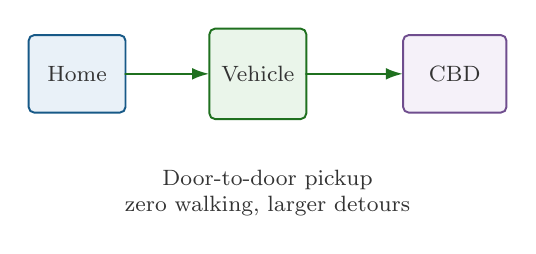
\begin{tikzpicture}[x=0.82cm,y=0.82cm]
\draw[home node] (0.2,1.8) rectangle (1.7,3.0);
\node[fig label] at (0.95,2.4) {Home};
\draw[vehicle node] (3.0,1.7) rectangle (4.5,3.1);
\node[fig label] at (3.75,2.4) {Vehicle};
\draw[cbd node] (6.0,1.8) rectangle (7.6,3.0);
\node[fig label] at (6.8,2.4) {CBD};
\draw[fig flow,draw=tabgreen!70!black] (1.7,2.4) -- (3.0,2.4);
\draw[fig flow,draw=tabgreen!70!black] (4.5,2.4) -- (6.0,2.4);
\node[fig label] at (3.9,0.55) {Door-to-door pickup\\zero walking, larger detours};
\end{tikzpicture}
\par\smallskip
\small (a) Home pickup
\end{minipage}\hfill
\begin{minipage}{0.47\textwidth}
\centering
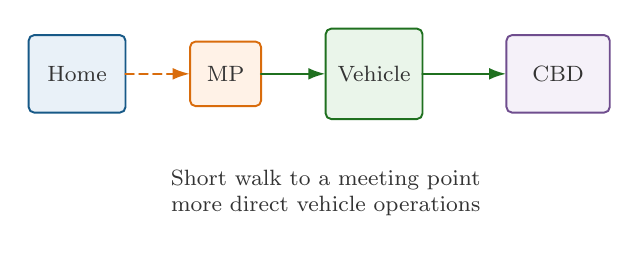
\begin{tikzpicture}[x=0.82cm,y=0.82cm]
\draw[home node] (0.2,1.8) rectangle (1.7,3.0);
\node[fig label] at (0.95,2.4) {Home};
\draw[mp node] (2.7,1.9) rectangle (3.8,2.9);
\node[fig label] at (3.25,2.4) {MP};
\draw[vehicle node] (4.8,1.7) rectangle (6.3,3.1);
\node[fig label] at (5.55,2.4) {Vehicle};
\draw[cbd node] (7.6,1.8) rectangle (9.2,3.0);
\node[fig label] at (8.4,2.4) {CBD};
\draw[fig dashed,draw=taborange!85!black] (1.7,2.4) -- (2.7,2.4);
\draw[fig flow,draw=tabgreen!70!black] (3.8,2.4) -- (4.8,2.4);
\draw[fig flow,draw=tabgreen!70!black] (6.3,2.4) -- (7.6,2.4);
\node[fig label] at (4.8,0.55) {Short walk to a meeting point\\more direct vehicle operations};
\end{tikzpicture}
\par\smallskip
\small (b) Walking to a recommended meeting point
\end{minipage}
\caption{Home pickup versus walking to recommended meeting points in many-to-one DRT. Home pickup eliminates walking but generally increases detours and service time, whereas meeting points trade a moderate walking burden for more direct vehicle operations.}
\label{fig:boarding-modes}
\end{figure}

Figure~\ref{fig:boarding-modes} contrasts the two boarding modes considered in the paper. Because final vehicle routes are only determined after all booking decisions have been made, the system must estimate the operational implications of each current decision under demand uncertainty and evolving capacity conditions. Figure~\ref{fig:interface} illustrates the passenger-facing menu.

\begin{figure}[t]
\centering
\begingroup
\setlength{\fboxsep}{8pt}
\fcolorbox{journalline}{white}{%
\begin{minipage}{0.84\textwidth}
\centering
\textbf{\footnotesize Current booking request}\\[5pt]
\renewcommand{\arraystretch}{1.15}
\begin{tabular}{lccc}
\toprule
Option & Fare adjustment & Walking distance & Predicted in-vehicle time \\
\midrule
Home pickup & \textcolor{tabred}{+2.0} & 0 m & 24 min \\
Meeting point A & \textcolor{tabgreen!70!black}{-5.0} & 280 m & 19 min \\
Meeting point B & \textcolor{tabgreen!70!black}{-3.0} & 150 m & 21 min \\
\bottomrule
\end{tabular}\\[6pt]
\footnotesize\textcolor{black!70}{A passenger chooses one internal option or rejects the offer.}
\end{minipage}}
\endgroup
\caption{Illustrative passenger menu with option-specific fare adjustment, walking distance, and predicted in-vehicle travel time.}
\label{fig:interface}
\end{figure}

\subsection{Decision timeline}

The booking process is modeled as a sequence of discrete decision epochs over a fixed booking horizon $[0,1,\ldots,T]$, where $T$ is the booking deadline. After time $T$, no additional requests are accepted and the operator solves the final multi-vehicle routing problem using the realized bookings. Passenger requests arrive sequentially at epochs $t=1,\ldots,T$, with origins drawn from the service-area distribution.

At each epoch, the online interaction unfolds as follows:
\begin{enumerate}
\item A passenger request arrives at epoch $t$.
\item The system recommends a set of boarding options, including home pickup and feasible meeting points, each with an associated price and predicted in-vehicle travel time.
\item The passenger either chooses an option $k \in O_t$ or rejects the service.
\item After the booking deadline $T$, the operator performs the final multi-vehicle routing optimization.
\end{enumerate}

\begin{figure}[t]
\centering
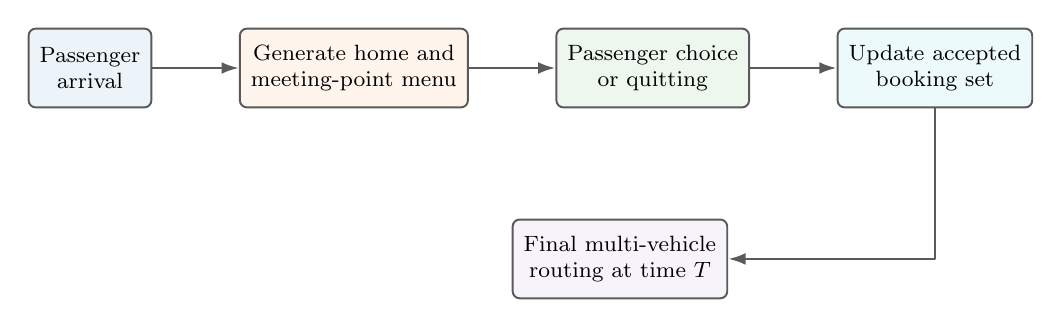
\begin{tikzpicture}[
node distance=1.3cm and 1.1cm,
]
\node[soft blue box] (arrive) {Passenger\\arrival};
\node[soft orange box,right=of arrive] (offer) {Generate home and\\meeting-point menu};
\node[soft green box,right=of offer] (choice) {Passenger choice\\or quitting};
\node[soft cyan box,right=of choice] (update) {Update accepted\\booking set};
\node[soft purple box,below=1.4cm of update,xshift=-4.0cm] (route) {Final multi-vehicle\\routing at time $T$};
\draw[fig flow] (arrive) -- (offer);
\draw[fig flow] (offer) -- (choice);
\draw[fig flow] (choice) -- (update);
\draw[fig flow] (update) |- (route);
\end{tikzpicture}
\caption{Online DRT workflow. Each arriving request triggers menu generation, pricing, passenger choice, booking-set update, and final routing after the booking horizon closes.}
\label{fig:workflow}
\end{figure}

For passenger $t$, the booking system offers home pickup $h_t$ and a set of recommended meeting points $M_t$, yielding the full option set $O_t = \{h_t\}\cup M_t$. For example, if $M_t = \{mp_1, mp_2, mp_3\}$, then $O_t = \{mp_1, mp_2, mp_3, h_t\}$. In the current implementation, $M_t$ is generated heuristically by selecting the $k$ closest meeting points to the passenger's home. Home pickup is always included so that passengers retain the option of doorstep service.

\subsection{Net-profit function}

The operator seeks to increase profit by steering some passengers from home pickup toward meeting points, thereby reducing routing costs without unduly reducing service acceptance. The operating cost contains four components: (i) labor cost associated with vehicle operating time, denoted by $c_{\omega}$; (ii) fuel cost associated with travel distance, denoted by $c_f$; (iii) expected cost of last-minute passenger cancellations, denoted by $c_m$; and (iv) the cost of traveling from the last served passenger's location to the common destination after all passengers have been served, denoted by $c_{\text{final}}$.

Passenger requests arrive sequentially, and the total number of arrivals follows an unknown demand process $D$. To capture behavioral heterogeneity, passengers are partitioned into segments $g\in\mathcal{G}$, where $\mu_g$ denotes the probability that an arriving passenger belongs to segment $g$.

Once the booking deadline is reached, the realized bookings and route plan are known. Let $B_T$ denote the accepted booking set at the end of the booking horizon, and let $R^T$ denote the corresponding route plan. The operator's objective is to maximize total net profit:
\begin{equation}
\max \; \Pi(B_T).
\tag{1}\label{eq:objective}
\end{equation}

\begin{align}
\Pi(B_T)={}&\sum_{(t,k)\in B_T}(f_e+a_{tk})
- c_{\omega}\left(\sum_{(i,j)\in \mathcal{A}(R^T)}\omega_{ij}
+\sum_{i\in \mathcal{N}(R^T)} l_i\right) \nonumber\\
&- c_f \sum_{(i,j)\in \mathcal{A}(R^T)} d_{ij}
- c_m\left[\rho_m \sum_{(t,k)\in B_T}\mathbf{1}\{k=h_t\}\right]
- c_{\text{final}}.
\tag{2}\label{eq:profit}
\end{align}

The first term in Eq.~\eqref{eq:profit} is total fare revenue, where $f_e$ is the base fare and $a_{tk}$ is the option-specific price adjustment. Negative values of $a_{tk}$ represent discounts, whereas positive values represent surcharges. The second and third terms capture time-related and distance-related operating costs, respectively. The fourth term represents the expected cost of last-minute cancellations for home-pickup orders, and the last term captures the final-leg cost to the common destination.

In the implementation used for the experiments, the service-time term distinguishes home pickup and meeting points. Home pickup incurs a base service time plus address-specific time, denoted by $l_0^{\mathrm{home}} + l_{\mathrm{addr}}(i)$, whereas a meeting point incurs a shorter fixed service time $l_{\mathrm{mp}}$. The default values are $l_0^{\mathrm{home}} = 2.5$ minutes and $l_{\mathrm{mp}} = 0.75$ minutes; Appendix~\ref{app:addl} reports all calibrated parameters.

\subsection{Dynamic programming formulation}

The online booking problem is inherently dynamic. Before the deadline $T$, the operator does not know how many additional passengers will arrive or how those future requests will alter the routing value of the current decision. Assigning the present passenger to one boarding option rather than another changes the future state of the system and may alter the downstream routing configuration. This interdependence motivates a Markov decision process formulation.

Let $V_t(s_t)$ denote the maximum expected cumulative profit from epoch $t$ to the end of the booking horizon, given state $s_t$. Because routing costs are realized only after the booking horizon closes, the terminal value is defined by the final routing cost:
\begin{equation}
V_{T+1}(s_{T+1}) = - C_T(B_T).
\tag{3}\label{eq:terminal}
\end{equation}

At epoch $t$, a passenger arrives with probability $\lambda_t \in [0,1]$, and no passenger arrives with probability $1-\lambda_t$. The state is written as
\begin{equation}
s_t = (B_{t-1},\xi_t),
\tag{4}\label{eq:state}
\end{equation}
where $B_{t-1}$ is the accepted booking set before epoch $t$ and $\xi_t$ is the information observed at that epoch. If a passenger arrives, then $\xi_t = (h_t,g_t)$, where $h_t$ is the home location and $g_t$ is the passenger segment; otherwise, $\xi_t=\varnothing$.

Conditional on an arrival, the recommendation module generates the option set $O_t$, and the operator selects the pricing vector $\mathbf{a}_t=(a_{tk})_{k\in O_t}$. Passenger choice then follows the multinomial logit model developed in Section~\ref{subsec:choice}. If the passenger selects an internal option $k\in O_t$, the booking set is updated; otherwise, it remains unchanged. The state transition is therefore
\begin{equation}
s_{t+1} =
\begin{cases}
s_t \oplus k, & \text{if passenger } t \text{ chooses } k \in O_t,\\
s_t, & \text{if the outside option is chosen or no passenger arrives.}
\end{cases}
\tag{5}\label{eq:transition}
\end{equation}

Since downstream routing costs are handled in the terminal value, the immediate reward at epoch $t$ contains only the fare collected from the current passenger. Let $f_e$ denote the base fare. Then the expected one-period reward for a passenger from segment $g_t$ is
\begin{equation}
r_t(\mathbf{a}_t) = \sum_{k\in O_t}(f_e+a_{tk})P_{tkg}(\mathbf{a}_t).
\tag{6}\label{eq:reward}
\end{equation}

\begin{align}
V_t(s_t)=\max_{\mathbf{a}_t}\Big\{&
\lambda_t \Big[\sum_{k\in O_t} P_{tkg}(\mathbf{a}_t)\big((f_e+a_{tk})+V_{t+1}(s_t\oplus k)\big) \nonumber\\
&\quad + P_{t0g}(\mathbf{a}_t) V_{t+1}(s_t)\Big]
+(1-\lambda_t)V_{t+1}(s_t)\Big\}.
\tag{7}\label{eq:bellman}
\end{align}

Directly solving Eq.~\eqref{eq:bellman} is computationally intractable because the state space expands rapidly with the evolving booking pattern and uncertain future arrivals. Even when the offered set is generated by a fixed heuristic, the marginal routing impact of the current choice still depends on future demand. The paper therefore adopts an approximate dynamic programming perspective and reinterprets the downstream value of each boarding option through its marginal contribution to final routing cost. This leads to a tractable per-passenger expected-profit problem, which is developed in Section~\ref{sec:method}.

\subsection{Passenger choice model}
\label{subsec:choice}

Passenger behavior is modeled with a multinomial logit specification. When a passenger arrives at epoch $t$, the operator presents the option set $O_t$ together with the corresponding price vector $\mathbf{a}_t=(a_{tk})_{k\in O_t}$. The passenger then chooses among the internal options and the outside option.

To capture heterogeneous preferences, passengers are partitioned into segments $g\in\mathcal{G}$. These segments differ in their sensitivities to walking distance, price, and in-vehicle travel time, with corresponding parameters $\beta_g^{\mathrm{walk}}$, $\beta_g^{\mathrm{price}}$, and $\beta_g^{\mathrm{ivt}}$. The outside option is characterized by a segment-specific baseline utility constant $U_{0g}$.

For a passenger in segment $g$, the utility of internal option $k\in O_t$ is
\begin{equation}
U_{tkg} = -\beta_g^{\mathrm{ivt}}\tau_{tk}
-\beta_g^{\mathrm{walk}}d_{tk}
-\beta_g^{\mathrm{price}}a_{tk}
\,+ \varepsilon_{tk}.
\tag{8}\label{eq:utility}
\end{equation}

Because $\beta_g^{\mathrm{ivt}} > 0$, $\beta_g^{\mathrm{walk}} > 0$, and $\beta_g^{\mathrm{price}} > 0$, shorter travel time, shorter walking distance, and a lower price all increase utility.

To capture the intrinsic preference for doorstep service, the calibrated experiments add a home-pickup alternative-specific constant $\alpha_g^{\mathrm{home}}$ to the home option. Operationally, this term is implemented as \texttt{home\_util}. Hence, for home pickup the model sets $d_{th_t}=0$ and writes
\[
U_{th_tg} =
\alpha_g^{\mathrm{home}}
- \beta_g^{\mathrm{ivt}}\tau_{th_t}
- \beta_g^{\mathrm{price}}a_{th_t}
+ \varepsilon_{th_t}.
\]

The meeting-point alternatives keep the normalized intercept equal to zero. The default calibration used in the experiments sets $\alpha_g^{\mathrm{home}} = 1.4$ and $U_{0g} = -1.0$.

The outside option is represented by
\begin{equation}
U_{t0g} = U_{0g} + \varepsilon_{t0}.
\tag{9}\label{eq:outside-utility}
\end{equation}

The disturbance terms $\varepsilon_{tk}$ and $\varepsilon_{t0}$ are assumed to be independently and identically distributed according to the Gumbel distribution, yielding the standard multinomial-logit structure. Here, $U_{0g}$ is the baseline utility of not using the offered service for segment $g$.

Under these assumptions, the probability that a passenger in segment $g$ chooses internal option $k$ is
\begin{equation}
P_{tkg}(\mathbf{a}_t)=
\frac{\exp\!\left[-\beta_g^{\mathrm{ivt}}\tau_{tk}
-\beta_g^{\mathrm{walk}}d_{tk}
-\beta_g^{\mathrm{price}}a_{tk}
+\mathbf{1}\{k=h_t\}\alpha_g^{\mathrm{home}}\right]}
{\exp(U_{0g})
+ \sum_{j\in O_t}\exp\!\left[-\beta_g^{\mathrm{ivt}}\tau_{tj}
-\beta_g^{\mathrm{walk}}d_{tj}
-\beta_g^{\mathrm{price}}a_{tj}
+\mathbf{1}\{j=h_t\}\alpha_g^{\mathrm{home}}\right]}.
\tag{10}\label{eq:choice-prob}
\end{equation}

The probability of choosing the outside option is
\begin{equation}
P_{t0g}(\mathbf{a}_t)=
\frac{\exp(U_{0g})}
{\exp(U_{0g})
+ \sum_{j\in O_t}\exp\!\left[-\beta_g^{\mathrm{ivt}}\tau_{tj}
-\beta_g^{\mathrm{walk}}d_{tj}
-\beta_g^{\mathrm{price}}a_{tj}
+\mathbf{1}\{j=h_t\}\alpha_g^{\mathrm{home}}\right]}.
\tag{11}\label{eq:outside-prob}
\end{equation}

These probabilities satisfy
\begin{equation}
P_{t0g}(\mathbf{a}_t)+\sum_{k\in O_t}P_{tkg}(\mathbf{a}_t)=1.
\tag{12}\label{eq:prob-sum}
\end{equation}

\section{Methodology}
\label{sec:method}

The DRPO framework combines a heuristic recommendation module, a predictive module for marginal insertion costs and pickup positions in the service sequence, and a pricing module trained with a decision-focused objective. In implementation terms, DRPO corresponds to the \texttt{DSPO\_plus\_SPO} variant of the original DSPO pipeline. The goal is to approximate the long-run routing impact of current decisions while preserving a tractable online implementation.

\subsection{Framework overview}

The core challenge in real-time DRT pricing is that the true marginal cost of assigning the current passenger to a specific boarding location depends on future passenger arrivals and on the final route plan, neither of which is known when the price must be quoted. DRPO addresses this challenge through an offline-online decomposition. Online, DRPO follows a recommend-predict-price pipeline. First, a heuristic recommendation module constructs the option set $O_t$ by retrieving the precomputed adjacency list of the $k$ closest feasible meeting points for the current home location ($k=10$ in the experiments) and adding the home-pickup option. Second, for each candidate option $k\in O_t$, the prediction module maps the option-level encoding $\phi(s_t,k)$ to an estimated marginal insertion cost and a pickup-position proxy, which together determine the displayed in-vehicle travel time. Third, conditional on the offered set and the predicted marginal costs, the pricing module determines the option-specific price vector $\mathbf{a}_t$ to maximize expected profit. Offline, the same framework generates counterfactual routing labels and trains the prediction model with a blended pointwise and decision-focused objective.

\begin{figure}[t]
\centering
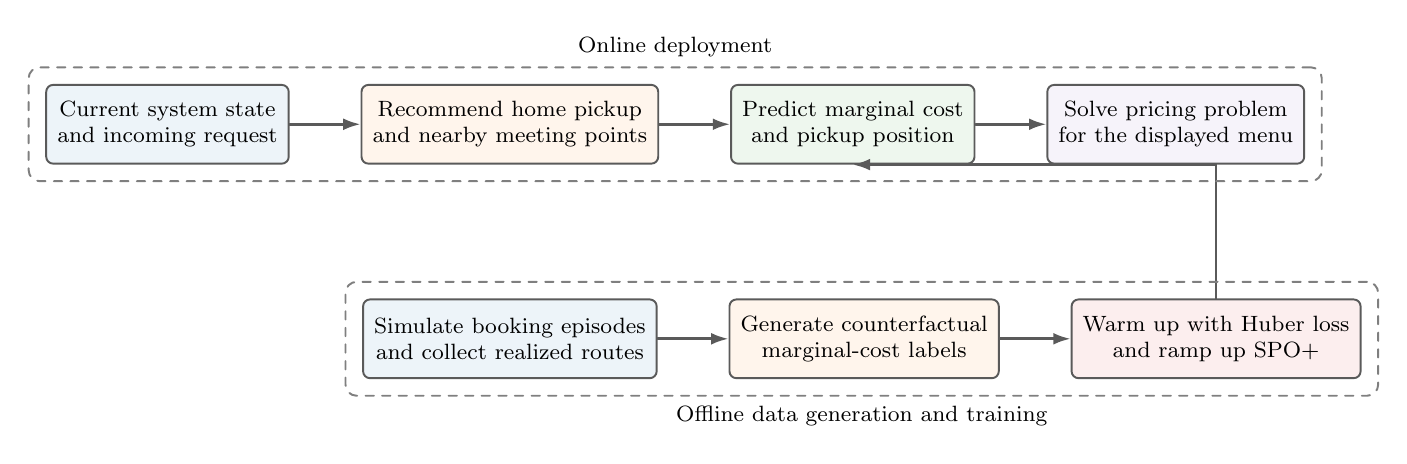
\begin{tikzpicture}[
node distance=1.2cm and 0.9cm,
]
\node[soft blue box] (state) {Current system state\\and incoming request};
\node[soft orange box,right=of state] (rec) {Recommend home pickup\\and nearby meeting points};
\node[soft green box,right=of rec] (pred) {Predict marginal cost\\and pickup position};
\node[soft purple box,right=of pred] (price) {Solve pricing problem\\for the displayed menu};
\node[soft blue box,below=1.7cm of rec] (sim) {Simulate booking episodes\\and collect realized routes};
\node[soft orange box,right=of sim] (labels) {Generate counterfactual\\marginal-cost labels};
\node[soft red box,right=of labels] (train) {Warm up with Huber loss\\and ramp up SPO+};
\draw[fig flow] (state) -- (rec);
\draw[fig flow] (rec) -- (pred);
\draw[fig flow] (pred) -- (price);
\draw[fig flow] (sim) -- (labels);
\draw[fig flow] (labels) -- (train);
\draw[fig flow] (train.north) |- (pred.south);
\node[journal group,fit=(state)(rec)(pred)(price),label=above:{\footnotesize Online deployment}] {};
\node[journal group,fit=(sim)(labels)(train),label=below:{\footnotesize Offline data generation and training}] {};
\end{tikzpicture}
\caption{Overview of the DRPO framework. The online layer recommends feasible boarding options, predicts option-level routing impact, and solves the pricing problem for the current passenger. The offline layer generates counterfactual routing labels and updates the predictive model with pointwise and decision-focused losses.}
\label{fig:framework}
\end{figure}

To obtain a tractable online decision problem, the dynamic program is reformulated as a per-passenger expected-profit problem in which the routing impact of each candidate option is represented by its marginal cost. Following \citet{yang2016}, the derivation from the Bellman equation is presented in Appendix~\ref{app:bellman}. Algorithm~1 summarizes the implementation workflow used in the experiments.

\noindent\textbf{Algorithm 1. Offline-online training and deployment procedure of DRPO}
\begin{enumerate}
\item Precompute, for each home location, the adjacency set of the $k$ nearest meeting points and initialize the choice-model and cost parameters.
\item Simulate booking episodes under the calibrated demand model and, for each decision epoch $t$, enumerate the feasible boarding options $O_t = \{h_t\}\cup M_t$.
\item For every candidate option $k\in O_t$, construct the option-level encoding $\phi(s_t,k)$ and generate a counterfactual routing label $c_{tk}$ by solving the terminal routing problem with and without the assignment of passenger $t$ to option $k$.
\item Train the marginal-cost predictor with a Huber loss during the initial phase; once the representation stabilizes, ramp up the SPO+ term and optimize the blended objective in Eq.~\eqref{eq:blend-loss}.
\item At deployment time, retrieve the feasible meeting-point set for the current passenger, predict option-level marginal costs and travel-time proxies, solve the pricing problem in Eq.~\eqref{eq:pricing-pred}, and display the resulting menu to the passenger.
\end{enumerate}

\subsection{State encoding and training data generation}

The first step is to convert the evolving DRT state into a representation suitable for machine learning. A spatiotemporal state representation is constructed that summarizes both where and when bookings have accumulated. Spatially, the service area is partitioned into grid cells. Temporally, the booking horizon is partitioned into equal-length intervals. Passenger arrivals are assigned to these intervals and aggregated accordingly. For each candidate boarding option $k\in O_t$, this state representation is paired with the focal option to form the option-level input $\phi(s_t,k)$. In implementation terms, $\phi(s_t,k)$ is an $n_{\text{layers}}\times X\times X$ tensor augmented with the remaining-capacity feature of the focal option. The default experiments use an $11\times 11$ spatial grid and two temporal layers.

\begin{figure}[t]
\centering
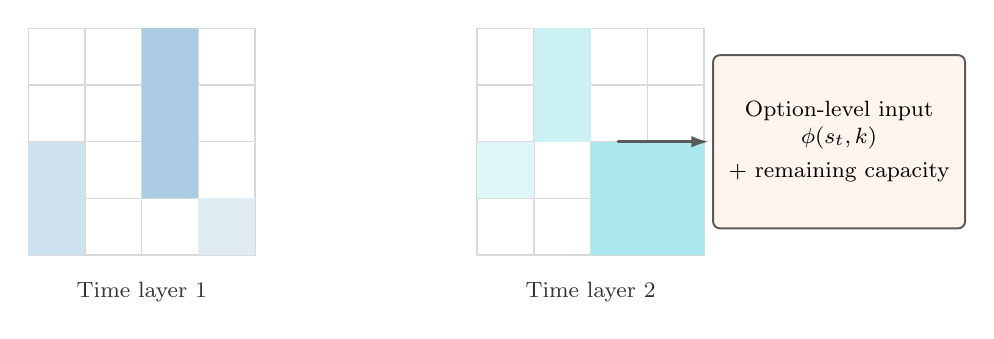
\begin{tikzpicture}[x=0.72cm,y=0.72cm]
\foreach \x in {0,...,4} {\draw[grid line] (\x,0) -- (\x,4);}
\foreach \y in {0,...,4} {\draw[grid line] (0,\y) -- (4,\y);}
\fill[tabblue!22] (0,0) rectangle (1,2);
\fill[tabblue!38] (2,1) rectangle (3,4);
\fill[tabblue!14] (3,0) rectangle (4,1);
\node[fig label] at (2,-0.65) {Time layer 1};
\begin{scope}[xshift=5.7cm]
\foreach \x in {0,...,4} {\draw[grid line] (\x,0) -- (\x,4);}
\foreach \y in {0,...,4} {\draw[grid line] (0,\y) -- (4,\y);}
\fill[tabcyan!22] (1,2) rectangle (2,4);
\fill[tabcyan!36] (2,0) rectangle (4,2);
\fill[tabcyan!14] (0,1) rectangle (1,2);
\node[fig label] at (2,-0.65) {Time layer 2};
\end{scope}
\draw[fig flow] (10.4,2.0) -- (12.0,2.0);
\node[soft orange box,minimum width=3.2cm,minimum height=2.2cm] at (14.3,2.0) {Option-level input\\$\phi(s_t,k)$\\[3pt]\footnotesize + remaining capacity};
\end{tikzpicture}
\caption{State encoding. Passenger requests observed so far are aggregated into a spatiotemporal tensor indexed by grid cell and time interval, and then paired with the focal boarding option to form the option-level predictor input.}
\label{fig:encoding}
\end{figure}

Training labels are generated as option-specific marginal insertion costs. For each decision epoch $t$ and each candidate option $k\in O_t$, a counterfactual terminal instance is constructed in which passenger $t$ is assigned to option $k$ while the remaining realized bookings are unchanged. The associated routing problem is solved and compared with the corresponding instance without passenger $t$. The resulting cost difference is recorded as the true marginal insertion cost $c_{tk}$. Hence, each arriving passenger contributes one labeled sample for every candidate option, rather than only for the option ultimately chosen.

\begin{figure}[t]
\centering
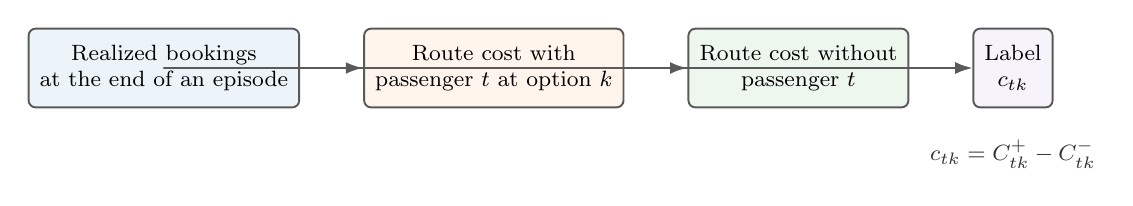
\begin{tikzpicture}[
node distance=1.3cm and 0.8cm,
]
\node[soft blue box] (realized) {Realized bookings\\at the end of an episode};
\node[soft orange box,right=of realized] (withk) {Route cost with\\passenger $t$ at option $k$};
\node[soft green box,right=of withk] (withoutk) {Route cost without\\passenger $t$};
\node[soft purple box,right=of withoutk] (diff) {Label\\$c_{tk}$};
\draw[fig flow] (realized) -- (withk);
\draw[fig flow] (realized) |- (withoutk);
\draw[fig flow] (withk) -- (diff);
\draw[fig flow] (withoutk) -- (diff);
\node[fig label,below=0.28cm of diff] {$c_{tk} = C^{+}_{tk} - C^{-}_{tk}$};
\end{tikzpicture}
\caption{Training data generation process. Each decision epoch yields one labeled sample per candidate option by comparing the terminal routing cost with and without the corresponding passenger-option assignment.}
\label{fig:labels}
\end{figure}

\subsection{Prediction module}

For each arriving passenger and each candidate boarding option $k\in O_t$, the system predicts two outputs: (i) the marginal operational cost used in pricing, and (ii) the predicted pickup position in the service sequence, which is used to calculate in-vehicle travel time. In the implementation used for the experiments, these quantities are produced by two parallel convolutional predictors that share the same option-level input specification. Each predictor contains two $3\times 3$ convolutional layers, one $2\times 2$ average-pooling layer, and two fully connected layers of width 256 and 128 with dropout 0.05. The remaining-capacity scalar of the focal option is concatenated before the first fully connected layer. This architecture is designed to extract hierarchical spatiotemporal patterns from the option-specific encoding $\phi(s_t,k)$ while keeping the online inference step lightweight.

Formally,
\begin{equation}
\left(\hat{c}_{tk}, \hat{q}_{tk}\right) = \mathcal{N}_{\theta}\!\left(\phi(s_t,k)\right),
\tag{13}\label{eq:nn}
\end{equation}
where $\mathcal{N}_{\theta}$ denotes the prediction network with parameters $\theta$. The predicted cost $\hat{c}_{tk}$ is passed directly to the pricing module, while the second output is used to derive the in-vehicle travel time shown to passengers.

\begin{figure}[t]
\centering
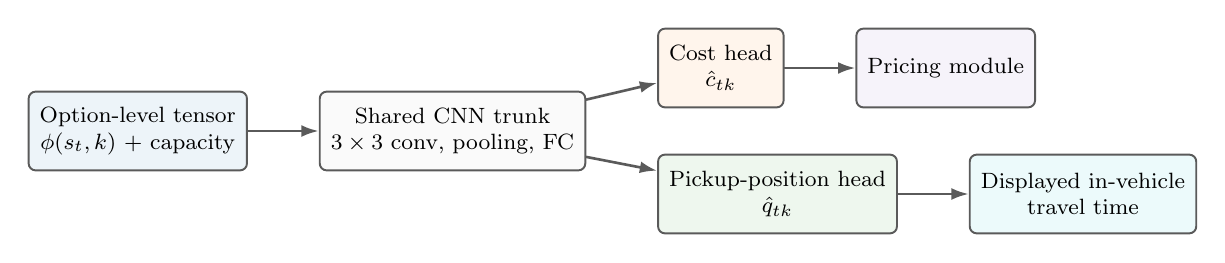
\begin{tikzpicture}[
node distance=1.3cm and 0.9cm,
]
\node[soft blue box] (input) {Option-level tensor\\$\phi(s_t,k)$ + capacity};
\node[soft gray box,right=of input] (cnn) {Shared CNN trunk\\$3\times 3$ conv, pooling, FC};
\node[soft orange box,right=of cnn,yshift=0.8cm] (cost) {Cost head\\$\hat{c}_{tk}$};
\node[soft green box,right=of cnn,yshift=-0.8cm] (pos) {Pickup-position head\\$\hat{q}_{tk}$};
\node[soft purple box,right=of cost] (pricing) {Pricing module};
\node[soft cyan box,right=of pos] (ivt) {Displayed in-vehicle\\travel time};
\draw[fig flow] (input) -- (cnn);
\draw[fig flow] (cnn) -- (cost);
\draw[fig flow] (cnn) -- (pos);
\draw[fig flow] (cost) -- (pricing);
\draw[fig flow] (pos) -- (ivt);
\end{tikzpicture}
\caption{Prediction module for marginal cost and in-vehicle travel time. The same option-level encoding is used to estimate marginal insertion costs for pricing and a service-sequence proxy for the displayed in-vehicle travel time.}
\label{fig:predictor}
\end{figure}

\subsection{Pricing optimization based on predicted costs}

Once the option set $O_t$ has been generated and the marginal costs have been predicted, the operator solves a real-time pricing problem for the current passenger. Consider a passenger from segment $g$ arriving at epoch $t$, with option set $O_t$ and price vector $\mathbf{a}_t=(a_{tk})_{k\in O_t}$. If the true marginal insertion cost of assigning the passenger to option $k$ is $c_{tk}$, then the expected-profit maximization problem is
\begin{equation}
\max_{\mathbf{a}_t} \sum_{k\in O_t} \left(f_e+a_{tk}-c_{tk}\right) P_{tkg}(\mathbf{a}_t).
\tag{14}\label{eq:pricing-true}
\end{equation}

The operational difficulty is that $c_{tk}$ is not observable when the pricing decision is made, because it depends on future arrivals and on the final routing plan. DRPO therefore replaces $c_{tk}$ with the predicted marginal insertion cost $\hat{c}_{tk}$ produced by the neural network, yielding the practical online problem
\begin{equation}
\max_{\mathbf{a}_t} \sum_{k\in O_t} \left(f_e+a_{tk}-\hat{c}_{tk}\right) P_{tkg}(\mathbf{a}_t).
\tag{15}\label{eq:pricing-pred}
\end{equation}

To streamline the derivation, suppress the time and segment indices and focus on a single passenger. Let $O$ denote the set of available options, let $a_k$ be the price adjustment for option $k\in O$, and let $\mathbf{a}=(a_k)_{k\in O}$ be the pricing vector. Likewise, let $c_k$ and $\hat{c}_k$ denote the true and predicted marginal insertion costs, with vector forms $\mathbf{c}=(c_k)_{k\in O}$ and $\hat{\mathbf{c}}=(\hat{c}_k)_{k\in O}$. Let $P_k(\mathbf{a})$ denote the probability that option $k$ is selected. Then the true-cost and prediction-based objectives can be written as
\begin{equation}
R(\mathbf{a};\mathbf{c}) = \sum_{k\in O} (f_e+a_k-c_k)P_k(\mathbf{a}),
\tag{16}\label{eq:rtrue}
\end{equation}
and
\begin{equation}
R(\mathbf{a};\hat{\mathbf{c}}) = \sum_{k\in O} (f_e+a_k-\hat{c}_k)P_k(\mathbf{a}),
\tag{17}\label{eq:rhat}
\end{equation}
so that the ideal and practical pricing problems become
\begin{equation}
\max_{\mathbf{a}\in\mathcal{A}} R(\mathbf{a};\mathbf{c}),
\qquad
\max_{\mathbf{a}\in\mathcal{A}} R(\mathbf{a};\hat{\mathbf{c}}),
\tag{18}\label{eq:pricing-general}
\end{equation}
where $\mathcal{A}$ is the feasible price set. For any cost vector $\mathbf{c}$, let
\begin{equation}
\mathbf{a}^{*}(\mathbf{c}) \in \argmax_{\mathbf{a}\in\mathcal{A}} R(\mathbf{a};\mathbf{c}),
\tag{19}\label{eq:oracle}
\end{equation}
denote the optimal pricing decision. Likewise, for a predicted cost vector $\hat{\mathbf{c}}$, let
\begin{equation}
\mathbf{a}^{*}(\hat{\mathbf{c}}) \in \argmax_{\mathbf{a}\in\mathcal{A}} R(\mathbf{a};\hat{\mathbf{c}}).
\tag{20}\label{eq:oracle-hat}
\end{equation}

The mapping $\mathbf{c}\mapsto \mathbf{a}^{*}(\mathbf{c})$ functions as the downstream pricing oracle in DRPO.

\subsection{SPO decision-focused learning objective}

The prediction module is trained for decision quality rather than for prediction accuracy alone. A model that produces small pointwise errors in marginal costs can still induce poor prices if those errors distort the downstream optimization problem in decision-relevant directions. The paper therefore adopts the Smart Predict-Then-Optimize framework of \citet{elmachtoub2022}.

To align the pricing problem with the canonical SPO form, first rewrite the downstream problem as a linear-objective optimization problem. For a fixed passenger, let $\mathbf{c}=(c_k)_{k\in O}$ and $\hat{\mathbf{c}}=(\hat{c}_k)_{k\in O}$ denote the true and predicted marginal-cost vectors. The downstream pricing problem is
\begin{equation}
\max_{\mathbf{a}\in\mathcal{A}} R(\mathbf{a};\mathbf{c}).
\tag{21}\label{eq:spo-downstream}
\end{equation}

Define
\begin{equation}
R_0(\mathbf{a}) = \sum_{k\in O}(f_e+a_k)P_k(\mathbf{a}),
\qquad
\mathbf{P}(\mathbf{a}) = [P_k(\mathbf{a})]_{k\in O},
\tag{22}\label{eq:r0}
\end{equation}
so that
\begin{equation}
R(\mathbf{a};\mathbf{c}) = R_0(\mathbf{a}) - \mathbf{c}^{\top}\mathbf{P}(\mathbf{a}).
\tag{23}\label{eq:rlinear}
\end{equation}

Introduce the augmented cost vectors and lifted decision vector
\begin{equation}
\mathbf{c}_{\mathrm{aug}}=
\begin{bmatrix}
\mathbf{c}\\
1
\end{bmatrix},
\qquad
\hat{\mathbf{c}}_{\mathrm{aug}}=
\begin{bmatrix}
\hat{\mathbf{c}}\\
1
\end{bmatrix},
\qquad
\mathbf{w}(\mathbf{a})=
\begin{bmatrix}
\mathbf{P}(\mathbf{a})\\
-R_0(\mathbf{a})
\end{bmatrix}.
\tag{24}\label{eq:augmented}
\end{equation}

For compactness, let
\begin{equation}
\mathbf{y}=\mathbf{c}_{\mathrm{aug}},
\qquad
\hat{\mathbf{y}}=\hat{\mathbf{c}}_{\mathrm{aug}}.
\tag{25}\label{eq:ydef}
\end{equation}
Then, for any feasible $\mathbf{a}\in\mathcal{A}$,
\begin{equation}
\mathbf{y}^{\top}\mathbf{w}(\mathbf{a})
= \mathbf{c}^{\top}\mathbf{P}(\mathbf{a}) - R_0(\mathbf{a})
= -R(\mathbf{a};\mathbf{c}).
\tag{26}\label{eq:yw}
\end{equation}

Hence, maximizing downstream profit is equivalent to minimizing a linear objective:
\begin{equation}
\max_{\mathbf{a}\in\mathcal{A}} R(\mathbf{a};\mathbf{c})
\Longleftrightarrow
\min_{\mathbf{a}\in\mathcal{A}} \mathbf{y}^{\top}\mathbf{w}(\mathbf{a}).
\tag{27}\label{eq:spo-primal}
\end{equation}

Let $\mathcal{W}=\operatorname{conv}\{\mathbf{w}(\mathbf{a}): \mathbf{a}\in\mathcal{A}\}$ be the convex hull of all lifted feasible decisions, and define
\begin{equation}
z^{*}(\mathbf{y}) = \min_{\mathbf{w}\in\mathcal{W}} \mathbf{y}^{\top}\mathbf{w},
\qquad
\mathbf{w}^{*}(\mathbf{y}) \in \argmin_{\mathbf{w}\in\mathcal{W}} \mathbf{y}^{\top}\mathbf{w}.
\tag{28}\label{eq:zstar}
\end{equation}

The SPO loss measures the downstream regret incurred when pricing is based on the predicted rather than the true cost vector:
\begin{equation}
\ell_{\mathrm{SPO}}(\hat{\mathbf{y}},\mathbf{y})
= \mathbf{y}^{\top}\mathbf{w}^{*}(\hat{\mathbf{y}})
- z^{*}(\mathbf{y}).
\tag{29}\label{eq:spo-loss}
\end{equation}
Using Eq.~\eqref{eq:yw}, this can be written directly as the profit loss induced by prediction error:
\begin{equation}
\ell_{\mathrm{SPO}}(\hat{\mathbf{y}},\mathbf{y})
= R\big(\mathbf{a}^{*}(\mathbf{c});\mathbf{c}\big)
- R\big(\mathbf{a}^{*}(\hat{\mathbf{c}});\mathbf{c}\big).
\tag{30}\label{eq:spo-regret}
\end{equation}

Because $\ell_{\mathrm{SPO}}$ is generally nonconvex and nondifferentiable, the paper instead optimizes the convex surrogate $\ell_{\mathrm{SPO}+}$:
\begin{equation}
\ell_{\mathrm{SPO}+}(\hat{\mathbf{y}},\mathbf{y})
= \max_{\mathbf{w}\in\mathcal{W}} (\mathbf{y}-2\hat{\mathbf{y}})^{\top}\mathbf{w}
+ 2\hat{\mathbf{y}}^{\top}\mathbf{w}^{*}(\mathbf{y})
- z^{*}(\mathbf{y}).
\tag{31}\label{eq:spoplus}
\end{equation}

A valid subgradient with respect to the augmented prediction is
\begin{equation}
2\left(\mathbf{w}^{*}(\mathbf{y}) - \mathbf{w}^{*}(2\hat{\mathbf{y}}-\mathbf{y})\right)
\in \partial_{\hat{\mathbf{y}}}\ell_{\mathrm{SPO}+}(\hat{\mathbf{y}},\mathbf{y}).
\tag{32}\label{eq:spograd}
\end{equation}

Because the last component of $\hat{\mathbf{y}}$ is fixed at $1$, backpropagation is performed only through the first $|O|$ entries corresponding to $\hat{\mathbf{c}}$. To stabilize optimization, the decision-focused loss is combined with a Huber loss on marginal-cost prediction:
\begin{equation}
\mathcal{L}(\theta)
= \lambda_{\mathrm{SPO}+}\,\ell_{\mathrm{SPO}+}(\hat{\mathbf{y}},\mathbf{y})
+ (1-\lambda_{\mathrm{SPO}+})\,\mathcal{L}_{\mathrm{Huber}}(\hat{\mathbf{c}},\mathbf{c}).
\tag{33}\label{eq:blend-loss}
\end{equation}

The parameter $\lambda_{\mathrm{SPO}+}\in[0,1]$ balances downstream decision quality against pointwise prediction accuracy. In a warm-up phase, training relies on the Huber loss alone to learn stable spatial and cost representations. The weight on the SPO+ term is then gradually increased, allowing the model to shift toward decision-focused learning without destabilizing early-stage optimization.

\section{Results}
\label{sec:results}

This section evaluates three questions. First, how does DRPO compare with simple operational extremes and static pricing? Second, does the SPO extension improve over the original DSPO objective under matched random seeds? Third, are the findings robust to alternative behavioral parameters and fleet sizes?

\subsection{Experimental design}

All experiments consider a many-to-one DRT service in which passengers travel from dispersed origins to a common destination. All strategies are evaluated under the same default demand and passenger-choice assumptions, including the outside option, so passenger quitting remains endogenous to the pricing policy. The paper reports operator-side outcomes, such as total cost and net profit, together with demand-side outcomes, such as the home-pickup share and quit rate. Tables in the main text report mean $\pm$ standard deviation across seeds; for key comparisons, the text also quotes 95\% confidence-interval half widths from the seed-level summaries.

The synthetic benchmark compares six policies:
\begin{itemize}
\item \texttt{Only-home}: home pickup only.
\item \texttt{Only-meeting-points}: meeting points only.
\item \texttt{No-pricing}: both boarding modes are available, but no price adjustments are applied.
\item \texttt{Static-pricing}: a fixed home-pickup surcharge and fixed meeting-point discount.
\item \texttt{DSPO}: the original learning-based pricing method adapted from \citet{akkerman2025}.
\item \texttt{DRPO}: DSPO augmented with SPO-based decision-focused training; in the codebase, this method is implemented as \texttt{DSPO\_plus\_SPO}.
\end{itemize}

The Beijing case study keeps \texttt{Static-pricing}, \texttt{DSPO}, and \texttt{DRPO} in the main table, while Appendix~\ref{app:addl} reports the remaining 25-vehicle baselines and the 15- and 40-vehicle robustness checks. Default demand, cost, learning, and choice-model parameters are summarized in Table~\ref{tab:d1}. The synthetic benchmark uses 30 seeds. The Beijing 25-vehicle case uses five seeds (40, 67, 97, 123, 456), and the 15- and 40-vehicle robustness checks use three seeds (40, 67, 97).

\subsection{Synthetic case}

\subsubsection{Problem setting}

The synthetic benchmark is based on the Gehring-Homberger instance family \citep{homberger2005}. It generates 200 geographic locations and splits them into disjoint training and test sets of 100 locations each. From each set, 10 locations are sampled as candidate meeting points. Figure~\ref{fig:synthetic-layout} provides a stylized visualization of the dispersed spatial layout used to generate these instances.

Driving times are based on Euclidean distances. Vehicle speed is set to 30 distance units per hour, the driver wage to 30 per hour, fuel cost to 0.6 per distance unit, home-pickup failure probability to 0.1, and the failure penalty to 20 per occurrence. Revenue per served passenger is fixed at 50 across all scenarios.

\begin{figure}[t]
\centering
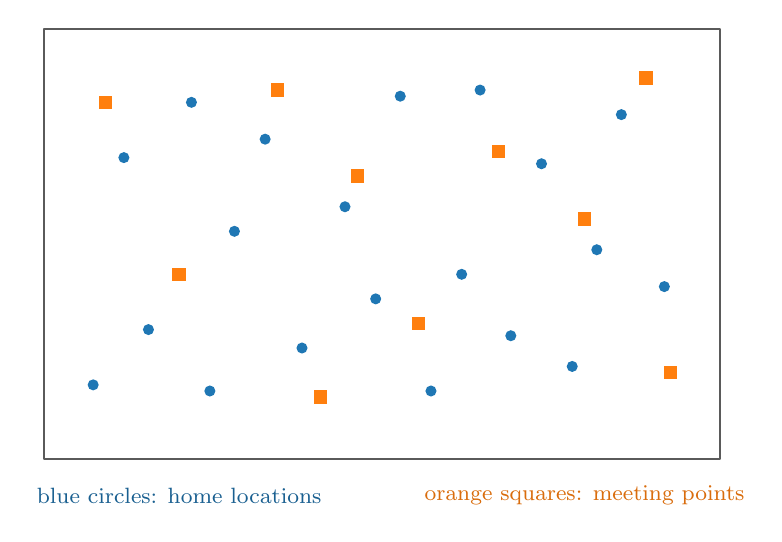
\begin{tikzpicture}[x=0.78cm,y=0.78cm]
\draw[journalline, line width=0.7pt] (0,0) rectangle (11,7);
\foreach \x/\y in {0.8/1.2,1.3/4.9,1.7/2.1,2.4/5.8,2.7/1.1,3.1/3.7,3.6/5.2,4.2/1.8,4.9/4.1,5.4/2.6,5.8/5.9,6.3/1.1,6.8/3.0,7.1/6.0,7.6/2.0,8.1/4.8,8.6/1.5,9.0/3.4,9.4/5.6,10.1/2.8} {
\fill[tabblue] (\x,\y) circle (2.0pt);
}
\foreach \x/\y in {1.0/5.8,2.2/3.0,3.8/6.0,5.1/4.6,6.1/2.2,7.4/5.0,8.8/3.9,9.8/6.2,4.5/1.0,10.2/1.4} {
\fill[taborange] (\x-0.11,\y-0.11) rectangle (\x+0.11,\y+0.11);
}
\node[fig label,text=tabblue!80!black] at (2.2,-0.6) {blue circles: home locations};
\node[fig label,text=taborange!85!black] at (8.8,-0.6) {orange squares: meeting points};
\end{tikzpicture}
\caption{Stylized spatial layout of the synthetic benchmark. Blue circles denote sampled home locations and orange squares denote candidate meeting points; the exact realizations vary by seed, but the figure reflects the dispersed geometry used to generate the benchmark instances.}
\label{fig:synthetic-layout}
\end{figure}

Service times are spatially heterogeneous. Following a common multimodal test setting in the optimization literature, waiting times are generated from the six-hump camel-back function introduced by \citet{molga2005}:
\begin{equation}
l_i(x,y) = \left(4-2.1x^2+\frac{x^4}{3}\right)x^2 + xy + \left(-4+4y^2\right)y^2.
\tag{34}\label{eq:camel}
\end{equation}
Service times are truncated to the interval $l_i\in[1,10]$ minutes. Daily passenger demand follows a negative binomial distribution:
\begin{equation}
\Pr(D=d) = \binom{d+r_{\mathrm{nb}}-1}{d}(1-p_{\mathrm{nb}})^d p_{\mathrm{nb}}^{r_{\mathrm{nb}}},
\qquad
d=0,1,2,\ldots,
\tag{35}\label{eq:nb}
\end{equation}
where $r_{\mathrm{nb}}=90$, $p_{\mathrm{nb}}=0.5$, and $\mathbb{E}[D]=90$. Passenger arrival times are uniformly distributed over the booking horizon. The fleet contains 15 vehicles, each with capacity 12. Because revealed boarding-choice data are unavailable, passenger behavior is simulated using the multinomial logit model of Section~\ref{subsec:choice}.

\subsubsection{Analysis of results}

Learning-based methods are trained for 200 episodes, and Table~\ref{tab:synthetic} reports averages over 30 random seeds.

\begin{table}[t]
\centering
\caption{Results on the synthetic case (30 seeds; mean $\pm$ std).}
\label{tab:synthetic}
\small
\begin{tabular}{lcccc}
\toprule
Strategy & Home-pickup share (\%) & Quit rate (\%) & Total costs & Net profit \\
\midrule
Only-home & $99.00 \pm 1.00$ & $1.01 \pm 0.87$ & $2890.75 \pm 376.66$ & $1590.92 \pm 353.59$ \\
Only-meeting-points & $0.00 \pm 0.00$ & $45.23 \pm 5.64$ & $702.95 \pm 226.98$ & $1780.39 \pm 499.06$ \\
No-pricing & $98.00 \pm 1.00$ & $1.01 \pm 0.87$ & $2885.99 \pm 381.99$ & $1595.67 \pm 349.23$ \\
Static-pricing & $22.00 \pm 5.00$ & $1.20 \pm 0.90$ & $2382.40 \pm 351.06$ & $2090.93 \pm 386.10$ \\
DSPO & $53.66 \pm 5.89$ & $3.69 \pm 1.39$ & $2218.46 \pm 263.92$ & $2193.79 \pm 398.01$ \\
DRPO & $45.32 \pm 6.77$ & $3.11 \pm 1.46$ & $2093.06 \pm 288.26$ & $2346.10 \pm 407.66$ \\
\bottomrule
\end{tabular}
\end{table}

Table~\ref{tab:synthetic} clarifies the role of the benchmark policies. \texttt{Only-home} and \texttt{No-pricing} are nearly identical, confirming that, without explicit incentives, most passengers continue to prefer home pickup. \texttt{Only-meeting-points} produces the lowest routing burden but also an impractically high quit rate of 45.23\%, so its apparent efficiency comes from aggressive demand loss rather than a balanced service design. \texttt{Static-pricing} is therefore the relevant feasible baseline.

Among the feasible adaptive methods, DRPO attains the highest mean net profit and the lowest mean total cost in this benchmark. Relative to \texttt{Static-pricing}, it reduces mean total cost by 12.14\% and increases mean net profit by 12.20\%. Relative to \texttt{DSPO}, it increases mean net profit by 6.94\%, reduces mean total cost by 5.65\%, lowers the home-pickup share from 53.66\% to 45.32\%, and lowers the quit rate from 3.69\% to 3.11\%. In the paired 30-seed comparison, DRPO yields higher net profit than DSPO on 29 seeds. The 95\% confidence-interval half widths for total cost are 131.07 for \texttt{Static-pricing}, 98.54 for \texttt{DSPO}, and 107.63 for \texttt{DRPO}, indicating that the improvement is not driven by a single outlying run.

These results suggest that the SPO-based training objective improves decision quality beyond both a strong static rule and the original DSPO objective. The gain is therefore attributable to better alignment between cost prediction and downstream pricing rather than to stronger price incentives alone.

\subsection{Yanjiao-Guomao case study in Beijing}

\subsubsection{Problem setting}

The case study focuses on the commuter corridor from Yanjiao to the Beijing central business district. Candidate meeting points are selected from 170 existing bus stops obtained from data published by the Beijing Municipal Transportation Commission.

Passenger demand is generated with parameters $r=240$ and $p=0.5$, so that $\mathbb{E}[D]=240$. In addition, 300 home locations are sampled according to a population-density distribution derived from official statistics for Beijing. The main experiments use 25 vehicles. Each vehicle has capacity 12. Revenue per served passenger is 50, and the pricing module searches over the interval $[-5,3.5]$. Driving times are again based on Euclidean distance. The remaining operating parameters match those of the synthetic case. For \texttt{Static-pricing}, the fixed home-pickup surcharge and meeting-point discount are set to 2 and 5, respectively. The 25-vehicle configuration is evaluated on five random seeds (40, 67, 97, 123, 456).

\begin{figure}[t]
\centering
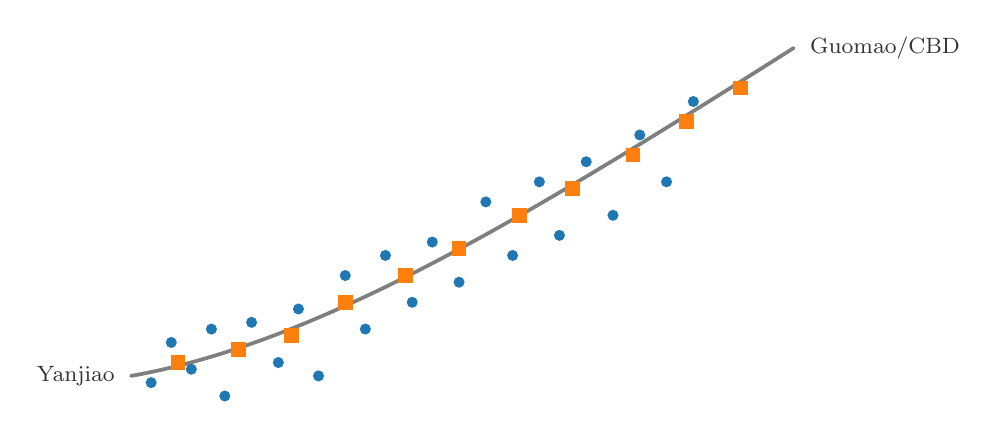
\begin{tikzpicture}[x=0.85cm,y=0.85cm]
\draw[tabgray, line width=1.35pt] (0.6,1.0) .. controls (3.4,1.5) and (6.4,3.3) .. (10.5,5.9);
\node[fig label,anchor=east] at (0.5,1.0) {Yanjiao};
\node[fig label,anchor=west] at (10.6,5.9) {Guomao/CBD};
\foreach \x/\y in {0.9/0.9,1.2/1.5,1.5/1.1,1.8/1.7,2.0/0.7,2.4/1.8,2.8/1.2,3.1/2.0,3.4/1.0,3.8/2.5,4.1/1.7,4.4/2.8,4.8/2.1,5.1/3.0,5.5/2.4,5.9/3.6,6.3/2.8,6.7/3.9,7.0/3.1,7.4/4.2,7.8/3.4,8.2/4.6,8.6/3.9,9.0/5.1} {
\fill[tabblue] (\x,\y) circle (2.0pt);
}
\foreach \x/\y in {1.3/1.2,2.2/1.4,3.0/1.6,3.8/2.1,4.7/2.5,5.5/2.9,6.4/3.4,7.2/3.8,8.1/4.3,8.9/4.8,9.7/5.3} {
\fill[taborange] (\x-0.11,\y-0.11) rectangle (\x+0.11,\y+0.11);
}
\end{tikzpicture}
\caption{Schematic corridor layout for the Beijing case. Blue circles denote sampled home locations and orange squares denote candidate bus-stop meeting points distributed along the Yanjiao--Guomao commuter corridor.}
\label{fig:beijing-layout}
\end{figure}

\subsubsection{Analysis of results}

Table~\ref{tab:beijing} reports the main results for the 25-vehicle Beijing configuration.

\begin{table}[t]
\centering
\caption{Main results on the semi-realistic Beijing case (5 seeds; mean $\pm$ std).}
\label{tab:beijing}
\small
\begin{tabular}{lcccc}
\toprule
Strategy & Home-pickup share (\%) & Quit rate (\%) & Total costs & Net profit \\
\midrule
Static-pricing & $25.05 \pm 2.21$ & $1.77 \pm 0.44$ & $3727.52 \pm 223.25$ & $7912.48 \pm 401.16$ \\
DSPO & $45.35 \pm 2.11$ & $4.04 \pm 0.64$ & $3717.28 \pm 277.18$ & $7656.22 \pm 385.03$ \\
DRPO & $37.18 \pm 3.67$ & $3.24 \pm 0.80$ & $3667.18 \pm 255.67$ & $7798.82 \pm 390.43$ \\
\bottomrule
\end{tabular}
\end{table}

The Beijing results are more nuanced than the synthetic benchmark and therefore provide a useful stress test. \texttt{Static-pricing} remains highly competitive and attains the highest mean net profit in this corridor. At the same time, DRPO achieves the lowest mean operating cost among the feasible policies in Table~\ref{tab:beijing} and improves on \texttt{DSPO}. Relative to \texttt{DSPO}, DRPO improves mean net profit by 1.86\%, reduces mean total cost by 1.35\%, lowers the home-pickup share from 45.35\% to 37.18\%, and lowers the quit rate from 4.04\% to 3.24\%. In the matched five-seed comparison, DRPO improves both total cost and net profit on all five seeds.

Compared with \texttt{Static-pricing}, DRPO reduces mean total cost by 1.62\% but accepts a 1.44\% reduction in mean net profit and a higher quit rate. The paper therefore does not claim that DRPO uniformly dominates every hand-tuned baseline in every metric. Instead, the Beijing evidence supports a narrower conclusion: adding SPO to DSPO improves the learning-based policy, and the resulting policy yields the lowest operating cost among the feasible Beijing policies evaluated in the current experiment set. The 95\% confidence-interval half widths for total cost are 195.69 for \texttt{Static-pricing}, 242.96 for \texttt{DSPO}, and 224.10 for \texttt{DRPO}; for net profit they are 351.63, 337.49, and 342.23, respectively.

Appendix~\ref{app:addl} provides two additional checks. Table~\ref{tab:d2} reports the full 25-vehicle benchmark set, showing that \texttt{Only-home} and \texttt{No-pricing} remain nearly identical in Beijing as well, whereas \texttt{Only-meeting-points} is operationally unrealistic because its quit rate exceeds 50\%. Table~\ref{tab:d3} reports 15- and 40-vehicle robustness results. Across those six matched seed pairs, DRPO improves mean profit at both fleet sizes and lowers mean cost in five of the six pairwise comparisons.

\subsection{Behavioral sensitivity analysis}

The sensitivity analysis revisits the behavioral robustness of the policy. Its purpose is not to claim universal superiority of DRPO, but to show when the method is most useful and when apparent cost savings mainly reflect demand loss. One parameter is varied at a time around the default calibration in Table~\ref{tab:d1}, and mean outcomes over three seeds are reported for each level.

\subsubsection{Effect of price sensitivity}

Figure~\ref{fig:price-sens} studies the magnitude of the price-sensitivity coefficient. When passengers become more responsive to price, the operator has more leverage to steer demand away from expensive home pickups and toward meeting points. Quantitatively, increasing the magnitude of the price coefficient from the default 0.25 to 0.35 raises mean net profit from 2414.06 to 3002.04, lowers mean total cost from 2010.94 to 1525.46, and lowers the mean quit rate from 4.06\% to 2.11\%.

\begin{figure}[t]
\centering
\includegraphics[width=0.82\textwidth]{fig11_beta_price_sensitivity}
\caption{Effect of the price-sensitivity coefficient on mean net profit, mean total cost, and mean quit rate relative to the default synthetic calibration.}
\label{fig:price-sens}
\end{figure}

This pattern is consistent with the role of price incentives: the more sensitive passengers are to discounts and surcharges, the easier it becomes to use pricing as a demand-steering instrument. When price sensitivity is weak, DRPO still functions, but the room for improvement is smaller because passenger choices become less elastic.

\subsubsection{Effect of outside-option utility}

Figure~\ref{fig:outside} studies the outside-option utility. This parameter captures how attractive it is for passengers to reject the DRT offer altogether and use another mode. The results show a sharp trade-off. Moving from the default $U_{0g}=-1.0$ to a neutral outside option around zero causes the mean quit rate to rise above 60\%, while the apparent reduction in total cost is largely driven by demand loss rather than by more efficient routing.

\begin{figure}[t]
\centering
\includegraphics[width=0.82\textwidth]{fig12_outside_option_sensitivity}
\caption{Effect of outside-option utility on mean net profit, mean total cost, and mean quit rate relative to the default synthetic calibration.}
\label{fig:outside}
\end{figure}

This result affects how the cost metric should be interpreted. Low operating cost is not automatically desirable when the outside option is highly attractive. In those settings, operator-side metrics should be read together with quit behavior and passenger retention.

\subsubsection{Effect of home-pickup preference}

Finally, Figure~\ref{fig:home} varies the home-pickup preference parameter \texttt{home\_util}, which operationalizes the home-pickup intercept $\alpha_g^{\mathrm{home}}$ introduced in Section~\ref{subsec:choice}. Reducing this parameter from the default 1.4 to 1.0 makes passengers more willing to walk. Mean total cost then falls from 2010.94 to 1441.40 and mean net profit rises from 2414.06 to 2795.26, but the mean quit rate also increases from 4.06\% to 8.48\%.

\begin{figure}[t]
\centering
\includegraphics[width=0.82\textwidth]{fig13_home_preference_sensitivity}
\caption{Effect of home-pickup preference on mean net profit, mean total cost, and mean quit rate relative to the default synthetic calibration.}
\label{fig:home}
\end{figure}

The implication is that weaker attachment to doorstep service creates more room for efficient meeting-point steering, but the induced efficiency gain may come with a nontrivial passenger-retention cost. The sensitivity analysis therefore complements the main experiments by showing that DRPO is most effective when passengers remain reasonably willing to substitute across boarding options and when the outside option is not too attractive.

\section{Conclusion}
\label{sec:conclusion}

This paper studies a sequential DRT decision problem that combines meeting-point recommendation with dynamic pricing in many-to-one systems. Unlike prior work that treats boarding behavior as fixed or focuses primarily on routing, the present framework explicitly models sequential passenger arrivals, heterogeneous choice behavior, and the trade-off between door-to-door convenience and system-wide operational efficiency.

The online problem is formulated as a Markov decision process in which the operator first generates a feasible set of boarding options and then assigns option-specific price incentives. To solve the resulting high-dimensional dynamic problem, the paper proposes DRPO, which combines heuristic meeting-point recommendation, spatiotemporal state encoding, marginal-cost prediction, and SPO+-based decision-focused learning. In implementation terms, DRPO is the SPO-augmented variant of DSPO and corresponds to \texttt{DSPO\_plus\_SPO} in the codebase.

The expanded experiments support three main observations. First, the extreme policies clarify the service trade-off: \texttt{Only-home} and \texttt{No-pricing} are nearly indistinguishable, whereas \texttt{Only-meeting-points} reduces routing burden only by triggering excessive quitting. Second, adding SPO to DSPO improves the learning-based policy. In the synthetic benchmark, DRPO outperforms both \texttt{Static-pricing} and \texttt{DSPO}; in the Beijing case, it improves on DSPO on every matched seed and achieves the lowest mean operating cost among the feasible policies evaluated in the current experiment set. Third, sensitivity analysis shows that the value of dynamic pricing depends strongly on passenger price sensitivity and on the attractiveness of the outside option.

These conclusions are intentionally narrower than the claims made in earlier drafts. The revised evidence does not imply that DRPO dominates every hand-tuned static rule on every metric in every scenario. Rather, it shows that the SPO extension improves DSPO in a stable way and provides a practically useful low-cost policy when the operator values routing efficiency and moderate passenger steering. At the same time, the current study relies on stylized travel times, a reduced-form passenger-choice model, and a many-to-one route structure with a common destination. The results should therefore be interpreted as evidence from the tested synthetic and Beijing settings rather than as a universal guarantee. Future work could extend the approach to endogenous meeting-point design, multi-destination and multimodal settings, richer routing constraints such as time windows and coordinated transfers, and field-calibrated behavioral data.

\section{Data and code availability}
\label{sec:data}

The experiment scripts and logs used for this revision are retained in the project workspace, but the current repository still contains legacy naming and auxiliary components inherited from an earlier out-of-home delivery codebase. To avoid making a misleading reproducibility claim, the paper does not cite the present workspace as a manuscript-aligned public replication package. Instead, this revision provides Algorithm~1, the calibrated parameter summary in Table~\ref{tab:d1}, seed-level variability summaries in Section~\ref{sec:results}, and supplementary benchmark tables in Appendix~\ref{app:addl}. A manuscript-aligned package containing the DRPO implementation, experiment scripts, seeds, and result tables will be released after the codebase has been cleaned and synchronized with the final paper version.

\appendix

\section{Notation}
\label{app:notation}

\subsection{Sets and indices}

\begin{itemize}
\item $\mathcal{G}$: set of passenger segments.
\item $g$: passenger-segment index.
\item $t$: decision epoch or request index.
\item $M_t$: set of recommended meeting-point options for passenger $t$; in the current implementation, it is generated from the precomputed set of the $k$ closest meeting points to the passenger's home.
\item $O_t$: full set of boarding options offered to passenger $t$, given by $O_t=\{h_t\}\cup M_t$.
\item $k$: boarding-option index in $O_t$.
\item $h_t$: home-pickup option for passenger $t$.
\item $0$: outside-option index.
\end{itemize}

\subsection{Cost, revenue, and routing variables}

\begin{itemize}
\item $f_e$: base fare.
\item $\mathbf{a}_t=(a_{tk})_{k\in O_t}$: price-adjustment vector for passenger $t$.
\item $a_{tk}$: price adjustment for option $k$ of passenger $t$.
\item $c_{tk}$: true marginal insertion cost.
\item $\hat{c}_{tk}$: predicted marginal insertion cost.
\item $c_{\omega}$: unit time-related operating cost.
\item $c_f$: unit distance-related operating cost.
\item $c_m$: unit cancellation cost.
\item $\rho_m$: cancellation probability for home-pickup orders.
\item $c_{\text{final}}$: final-leg cost to the common destination.
\item $l_0^{\mathrm{home}}$: fixed service-time component of a home pickup.
\item $l_{\mathrm{mp}}$: fixed service time at a meeting point.
\item $l_{\mathrm{addr}}(i)$: address-specific component of home-pickup service time at location $i$.
\item $C_T(B_T)$: terminal routing cost associated with the final accepted booking set.
\item $R^T$: final route plan after the booking horizon ends.
\item $\mathcal{A}(R^T)$: arc set of route plan $R^T$.
\item $\mathcal{N}(R^T)$: node set of route plan $R^T$.
\item $\omega_{ij}$: travel time on arc $(i,j)$.
\item $d_{ij}$: travel distance on arc $(i,j)$.
\item $l_i$: waiting time at node $i$.
\end{itemize}

The sign convention for pricing is $a_{tk}<0$ for a discount and $a_{tk}>0$ for a surcharge.

\subsection{Demand, state, and transition variables}

\begin{itemize}
\item $\Pr(\cdot)$: probability operator.
\item $\lambda_t$: passenger-arrival probability at epoch $t$.
\item $\mu_g$: probability that an arriving passenger belongs to segment $g$.
\item $\xi_t=(h_t,g_t)$: observed information of the arriving passenger at epoch $t$.
\item $s_t=(B_{t-1},\xi_t)$: system state at epoch $t$.
\item $s_t\oplus k$: updated state after passenger $t$ chooses internal option $k$.
\item $\phi(s_t,k)$: option-specific encoding formed by pairing system state $s_t$ with candidate boarding option $k$.
\item $B_t$: set of accepted bookings up to epoch $t$.
\item $B_T$: final accepted booking set at the booking deadline.
\end{itemize}

\subsection{Choice-model notation}

\begin{itemize}
\item $d_{tk}$: walking distance for passenger $t$ under option $k$.
\item $\tau_{tk}$: predicted in-vehicle travel time for passenger $t$ under option $k$.
\item $\hat{q}_{tk}$: predicted pickup position of passenger $t$ in the service sequence under option $k$.
\item $U_{tkg}$: utility of internal option $k$ for passenger $t$ in segment $g$.
\item $U_{t0g}$: utility of the outside option for passenger $t$ in segment $g$.
\item $\varepsilon_{tk}$: random disturbance term for internal option $k$.
\item $\varepsilon_{t0}$: random disturbance term for the outside option.
\item $\beta_g^{\mathrm{walk}}$: walking-distance sensitivity parameter for segment $g$.
\item $\beta_g^{\mathrm{price}}$: price-sensitivity parameter for segment $g$.
\item $\beta_g^{\mathrm{ivt}}$: in-vehicle-travel-time sensitivity parameter for segment $g$.
\item $\alpha_g^{\mathrm{home}}$: home-pickup alternative-specific constant; implemented as \texttt{home\_util} in the experiments.
\item $U_{0g}$: baseline utility of the outside option for segment $g$.
\item $P_{tkg}(\mathbf{a}_t)$: probability that passenger $t$ in segment $g$ chooses internal option $k$.
\item $P_{t0g}(\mathbf{a}_t)$: probability that passenger $t$ in segment $g$ chooses the outside option.
\end{itemize}

\subsection{Dynamic programming and profit notation}

\begin{itemize}
\item $r_t(\mathbf{a}_t)$: expected one-period revenue at epoch $t$.
\item $V_t(s_t)$: value function at epoch $t$ under state $s_t$.
\item $\Pi(B_T)$: total net profit associated with the final accepted booking set $B_T$.
\item $\Delta V_k(s_t)$: opportunity cost of assigning the current passenger to option $k$.
\item $R(\mathbf{a};\mathbf{c})$: downstream profit function under decision $\mathbf{a}$ and true cost vector $\mathbf{c}$.
\item $R_0(\mathbf{a})$: cost-independent revenue component in the reformulated downstream objective.
\end{itemize}

\subsection{Prediction and decision-focused learning notation}

\begin{itemize}
\item $\mathcal{N}_{\theta}$: prediction network used for marginal-cost and travel-time-proxy estimation.
\item $\mathbf{c}_{\mathrm{aug}}=[\mathbf{c}^{\top},1]^{\top}$: augmented true cost vector.
\item $\hat{\mathbf{c}}_{\mathrm{aug}}=[\hat{\mathbf{c}}^{\top},1]^{\top}$: augmented predicted cost vector.
\item $\mathbf{y} = \mathbf{c}_{\mathrm{aug}},\; \hat{\mathbf{y}} = \hat{\mathbf{c}}_{\mathrm{aug}}$: compact notation used in the SPO derivation.
\item $\mathbf{w}(\mathbf{a})=[\mathbf{P}(\mathbf{a})^{\top},-R_0(\mathbf{a})]^{\top}$: lifted decision vector induced by decision $\mathbf{a}$.
\item $\mathcal{W}$: convex hull of all lifted feasible decisions.
\item $z^{*}(\mathbf{y})$: optimal objective value under augmented cost vector $\mathbf{y}$.
\item $\mathbf{w}^{*}(\mathbf{y})$: optimal lifted decision under augmented cost vector $\mathbf{y}$.
\item $\ell_{\mathrm{SPO}}$: SPO regret loss.
\item $\ell_{\mathrm{SPO}+}$: SPO+ surrogate loss.
\end{itemize}

\section{Bellman-to-pricing derivation}
\label{app:bellman}

Starting from Eq.~\eqref{eq:reward}, consider a passenger arriving at epoch $t$ with option set $O_t$ and pricing vector $\mathbf{a}_t=(a_{tk})_{k\in O_t}$. If the passenger chooses internal option $k\in O_t$, the immediate reward is $f_e+a_{tk}$ and the continuation value is $V_{t+1}(s_t\oplus k)$. Therefore, the value of accepting the order through option $k$ is
\begin{equation}
\left(f_e+a_{tk}\right) + V_{t+1}(s_t\oplus k).
\tag{B.1}
\end{equation}

If the order is not accepted, or if the outside option is chosen, the state remains $s_t$ and the continuation value is $V_{t+1}(s_t)$. The net gain from accepting option $k$ is therefore
\begin{equation}
\left(f_e+a_{tk}\right) - \left[V_{t+1}(s_t) - V_{t+1}(s_t\oplus k)\right].
\tag{B.2}
\end{equation}

Define the opportunity cost
\begin{equation}
\Delta V_k(s_t) = V_{t+1}(s_t) - V_{t+1}(s_t\oplus k).
\tag{B.3}
\end{equation}

Under the multinomial logit model, the expected net profit at epoch $t$ can therefore be written as
\begin{equation}
\sum_{k\in O_t} P_{tkg}(\mathbf{a}_t)\left(f_e+a_{tk}-\Delta V_k(s_t)\right).
\tag{B.4}
\end{equation}

Given $\Delta V_k(s_t)$, maximizing the Bellman equation is equivalent to maximizing the expected net profit of the current passenger at each arrival epoch:
\begin{equation}
\max_{\mathbf{a}_t}
\sum_{k\in O_t} P_{tkg}(\mathbf{a}_t)\left(f_e+a_{tk}-\Delta V_k(s_t)\right).
\tag{B.5}
\end{equation}

The true opportunity cost $\Delta V_k(s_t)$ is not observable in real time because it depends on future arrivals and on the final route plan. The paper approximates it by the true marginal insertion cost $c_{tk}$, namely the change in total routing cost generated by inserting option $k$ into the final route. Substituting this approximation yields the per-passenger expected-profit problem reported in Eq.~\eqref{eq:pricing-true}:
\begin{equation}
\max_{\mathbf{a}_t}
\sum_{k\in O_t} (f_e+a_{tk}-c_{tk})P_{tkg}(\mathbf{a}_t).
\tag{B.6}
\end{equation}

\section{Analytical structure of the pricing problem}
\label{app:pricing}

For simplicity, fix a passenger segment $g$ and a decision epoch $t$, and suppress these subscripts whenever no confusion arises. Let $O$ denote the set of internal boarding options, and let $0$ denote the outside option. For each $k\in O$, define
\begin{equation}
\eta_k = -\beta_g^{\mathrm{ivt}}\tau_k - \beta_g^{\mathrm{walk}} d_k,
\qquad
\beta = \beta_g^{\mathrm{price}} > 0.
\tag{C.1}
\end{equation}

Then the multinomial logit choice probabilities can be written as
\begin{equation}
P_k(\mathbf{a}) =
\frac{\exp(\eta_k-\beta a_k)}
{\exp(U_{0g}) + \sum_{j\in O}\exp(\eta_j-\beta a_j)},
\qquad k\in O,
\tag{C.2}
\end{equation}
and
\begin{equation}
P_0(\mathbf{a}) =
\frac{\exp(U_{0g})}
{\exp(U_{0g}) + \sum_{j\in O}\exp(\eta_j-\beta a_j)}.
\tag{C.3}
\end{equation}

Given a true marginal insertion-cost vector $\mathbf{c}=(c_k)_{k\in O}$, the pricing problem is
\begin{equation}
\max_{\mathbf{a}\in\mathcal{A}} R(\mathbf{a};\mathbf{c})
=
\max_{\mathbf{a}\in\mathcal{A}} \sum_{k\in O}(f_e+a_k-c_k)P_k(\mathbf{a}).
\tag{C.4}
\end{equation}

Ignoring box constraints for a moment and considering an interior solution, define
\begin{equation}
g_k(\mathbf{a};\mathbf{c}) = f_e+a_k-c_k.
\tag{C.5}
\end{equation}
The first-order condition implies
\begin{equation}
g_k(\mathbf{a}^{*};\mathbf{c}) = R(\mathbf{a}^{*};\mathbf{c}) + \frac{1}{\beta},
\qquad \forall k\in O.
\tag{C.6}
\end{equation}

Equation~(C.6) shows that the optimal policy equalizes the net profit contribution across all internal options. Therefore, there exists a common markup term $m(\mathbf{c})$ such that
\begin{equation}
a_k^{*}(\mathbf{c}) = c_k - f_e + m(\mathbf{c}),
\qquad \forall k\in O.
\tag{C.7}
\end{equation}

Let
\begin{equation}
B(\mathbf{c}) = \sum_{j\in O}\exp(\eta_j-\beta c_j).
\tag{C.8}
\end{equation}
Then the total internal-choice probability can be written as
\begin{equation}
S(m;\mathbf{c}) =
\frac{\exp(\beta f_e-\beta m)B(\mathbf{c})}
{\exp(U_{0g}) + \exp(\beta f_e-\beta m)B(\mathbf{c})}.
\tag{C.9}
\end{equation}

Because Eq.~(C.7) implies $f_e + a_k^{*}(\mathbf{c}) - c_k = m(\mathbf{c})$ for every internal option $k$, the expected profit becomes
\begin{equation}
R\big(\mathbf{a}^{*}(\mathbf{c});\mathbf{c}\big)
=
m(\mathbf{c})\,S(m(\mathbf{c});\mathbf{c}).
\tag{C.10}
\end{equation}

Hence the multidimensional pricing problem reduces to
\begin{equation}
\max_m \; m\,S(m;\mathbf{c}).
\tag{C.11}
\end{equation}

The first-order condition implies
\begin{equation}
m(\mathbf{c}) =
\frac{1}{\beta\left(1-S(m(\mathbf{c});\mathbf{c})\right)}
=
\frac{1}{\beta P_0(\mathbf{a}^{*}(\mathbf{c}))}.
\tag{C.12}
\end{equation}

Finally, combining Eqs.~(C.7) and (C.12), the optimal price vector has the form
\begin{equation}
a_k^{*}(\mathbf{c})
=
c_k - f_e + m(\mathbf{c}),
\qquad
m(\mathbf{c}) = \frac{1}{\beta P_0(\mathbf{a}^{*}(\mathbf{c}))},
\quad \forall k\in O.
\tag{C.13}
\end{equation}

\section{Additional experimental details}
\label{app:addl}

\subsection{Default parameter summary}

\begin{table}[t]
\centering
\caption{Default parameter settings used in the revised experiments.}
\label{tab:d1}
\footnotesize
\begin{tabularx}{\textwidth}{lYY}
\toprule
Item & Synthetic benchmark & Beijing case \\
\midrule
Demand model & Negative binomial with $r=90$, $p=0.5$, $\mathbb{E}[D]=90$ & Negative binomial with $r=240$, $p=0.5$, $\mathbb{E}[D]=240$ \\
Candidate meeting-point pool & $k=10$ nearest meeting points per home location & $k=10$ nearest bus stops per home location \\
Spatial-temporal encoding & $11\times 11$ grid, $n_{\text{input layers}}=2$ & $11\times 11$ grid, $n_{\text{input layers}}=2$ \\
Fleet size & 15 vehicles & 25 vehicles in the main table; 15 and 40 in robustness checks \\
Vehicle capacity & 12 & 12 \\
Price bounds & $[-5,3.5]$ & $[-5,3.5]$ \\
Revenue per served passenger & 50 & 50 \\
Operating-cost parameters & Fuel cost 0.6, driver wage 30, $l_0^{\mathrm{home}}=2.5$ min, $l_{\mathrm{mp}}=0.75$ min, home-failure probability 0.1, failure penalty 20 & Same as synthetic \\
Choice-model defaults & \texttt{outside\_option\_util} $=-1.0$, \texttt{home\_util} $=1.4$, price-sensitivity magnitude 0.25 & Same as synthetic \\
Learning schedule & 200 episodes, initial phase 50, batch size 256, learning rate 0.001 & Same as synthetic \\
SPO schedule & Huber warm-up 5 episodes, SPO ramp-up 10 episodes, max SPO weight 0.7, phase-2 Huber weight 0.35 & Same as synthetic \\
Seeds & 30 seeds & Five seeds for the 25-vehicle case: 40, 67, 97, 123, 456; three seeds for the 15- and 40-vehicle robustness checks: 40, 67, 97 \\
\bottomrule
\end{tabularx}
\end{table}

\subsection{Supplementary Beijing baselines}

\begin{table}[t]
\centering
\caption{Additional 25-vehicle Beijing baseline results (mean $\pm$ std).}
\label{tab:d2}
\small
\begin{threeparttable}
\begin{tabular}{lccccc}
\toprule
Strategy & $n$ & Home-pickup share (\%) & Quit rate (\%) & Total costs & Net profit \\
\midrule
Only-home & 5 & $99.26 \pm 0.50$ & $0.74 \pm 0.50$ & $5115.22 \pm 262.97$ & $6644.78 \pm 314.32$ \\
Only-meeting-points & 4 & $0.00 \pm 0.00$ & $53.63 \pm 1.21$ & $473.23 \pm 165.71$ & $5089.27 \pm 557.26$ \\
No-pricing & 5 & $98.18 \pm 1.08$ & $0.74 \pm 0.50$ & $5093.67 \pm 243.78$ & $6666.33 \pm 334.29$ \\
Static-pricing & 5 & $25.05 \pm 2.21$ & $1.77 \pm 0.44$ & $3727.52 \pm 223.25$ & $7912.48 \pm 401.16$ \\
DSPO & 5 & $45.35 \pm 2.11$ & $4.04 \pm 0.64$ & $3717.28 \pm 277.18$ & $7656.22 \pm 385.03$ \\
DRPO & 5 & $37.18 \pm 3.67$ & $3.24 \pm 0.80$ & $3667.18 \pm 255.67$ & $7798.82 \pm 390.43$ \\
\bottomrule
\end{tabular}
\begin{tablenotes}
\footnotesize
\item Note: the available \texttt{Only-meeting-points} results contain four completed 25-vehicle Beijing runs; all other strategies contain five runs.
\end{tablenotes}
\end{threeparttable}
\end{table}

\subsection{Fleet-size robustness}

\begin{table}[t]
\centering
\caption{Beijing fleet-size robustness for DSPO and DRPO (mean $\pm$ std).}
\label{tab:d3}
\small
\begin{tabular}{lccccc}
\toprule
Fleet size & Strategy & Home-pickup share (\%) & Quit rate (\%) & Total costs & Net profit \\
\midrule
15 vehicles & DSPO & $45.30 \pm 1.56$ & $4.26 \pm 1.29$ & $2822.96 \pm 107.01$ & $5745.37 \pm 33.57$ \\
15 vehicles & DRPO & $36.64 \pm 1.12$ & $3.23 \pm 1.33$ & $2798.91 \pm 70.40$ & $5861.93 \pm 134.07$ \\
40 vehicles & DSPO & $46.64 \pm 1.72$ & $4.01 \pm 0.96$ & $3753.12 \pm 328.80$ & $7673.54 \pm 480.99$ \\
40 vehicles & DRPO & $37.33 \pm 2.03$ & $3.08 \pm 0.73$ & $3685.39 \pm 308.21$ & $7851.27 \pm 504.94$ \\
\bottomrule
\end{tabular}
\end{table}

Across the six matched robustness runs in Table~\ref{tab:d3}, DRPO improves profit in all six comparisons. It lowers total cost in two of the three 15-vehicle comparisons and in all three 40-vehicle comparisons, yielding lower mean cost at both fleet sizes.

\bibliographystyle{elsarticle-harv}
\bibliography{drpo_trc_refs}

\end{document}
